\documentclass[a4paper]{article}

%% Language and font encodings
\usepackage[english]{babel}
\usepackage[utf8x]{inputenc}
\usepackage[T1]{fontenc}

%% Sets page size and margins
\usepackage[a4paper,top=3cm,bottom=2cm,left=3cm,right=3cm,marginparwidth=1.75cm]{geometry}

%% Useful packages
\usepackage[colorinlistoftodos]{todonotes}
\usepackage[colorlinks=true, allcolors=blue]{hyperref}
\usepackage{subfig}
\usepackage{minted}

\title{Deep RL Arm Manipulation Writeup}
\author{Shingo Mori}

\begin{document}
\maketitle

This writeup addresses the rubric points for the fourth project of the Udacity Robotics Software Nanodegree Program Term 2.

\section{Introduction}
In this project, a robotic agent is created in a Gazebo environment and trained to touch the object of interest accurately within a certain amount of movements. The training is done in a reinforcement learning approach \cite{Sutton:1998:IRL:551283}, and the Deep Recurrent Q-Network (DRQN) \cite{Hausknecht2015}, a variant of the Deep Q-Network (DQN) \cite{Zhan2016}, is applied to determine the agent's action policy.

The main task of this project is to define a reward function and tune hyperparameters to carry out the following two primary objectives.

\begin{enumerate}
    \item Have any part of the robot arm touch the object of interest, with at least a 90\% accuracy for a minimum of 100 runs.
    \item Have only the gripper base of the robot arm touch the object, with at least a 80\% accuracy for a minimum of 100 runs.
\end{enumerate}

The environment is composed of an object of interest, a robotic arm to touch the object and a camera to observe the state of the environment. An image of the environment setup is shown in Figure \ref{fig:environment}.

\begin{figure}[ht]
\centering
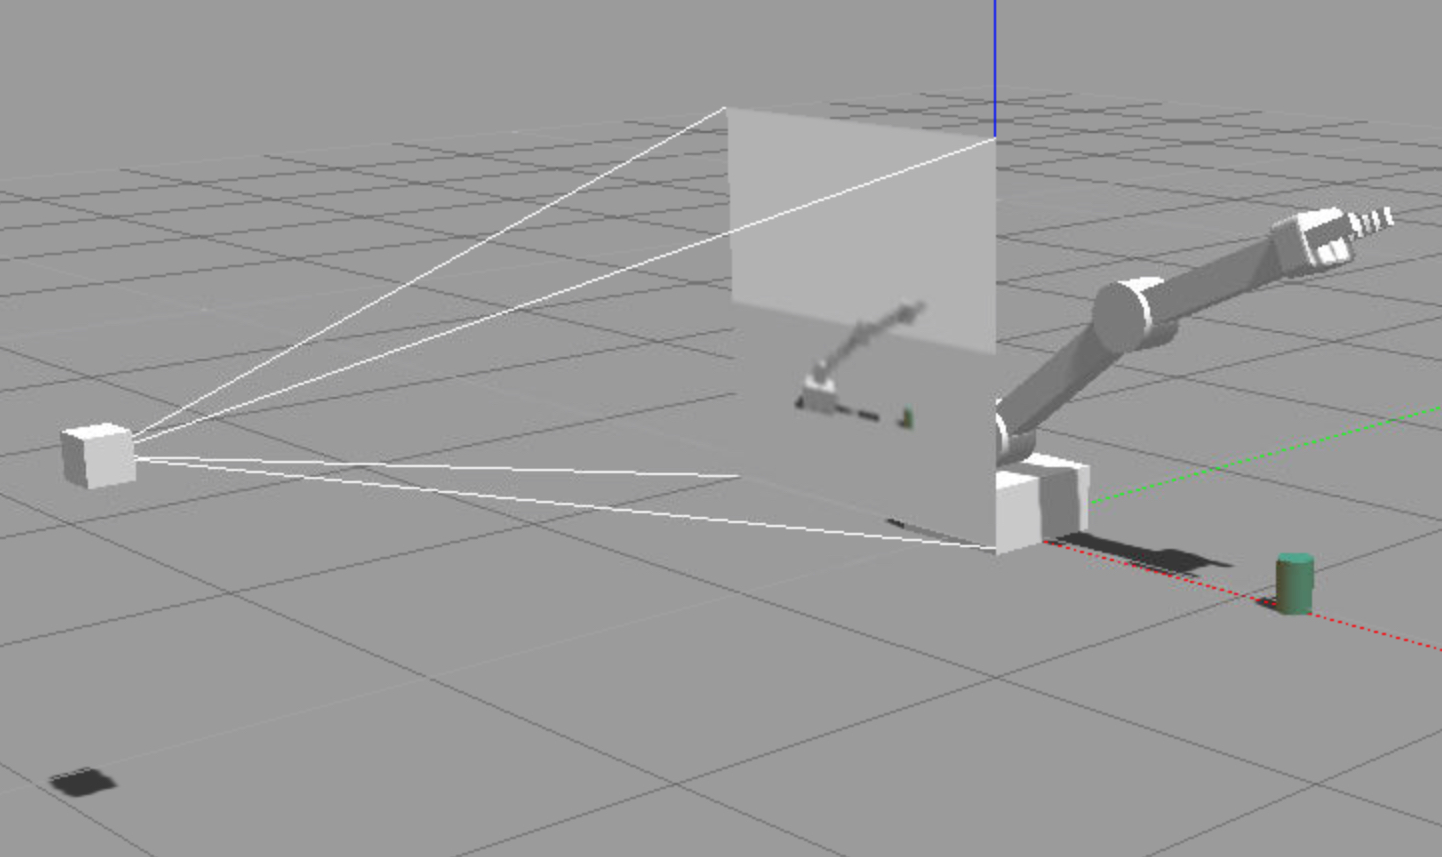
\includegraphics[width=0.6\textwidth]{environment}
\caption{Gazebo environment setup. }
\label{fig:environment}
\end{figure}

\section{Reward Function}
\subsection{Action Command}
The robotic arm has three revolute joints. The agent manipulates those joints by sending an action command every frame. In this project, there are two options we can choose for what action to send to control those joints. We can either send a velocity-control action to specify the angular velocity of a joint, or send an angle-control action to specify the angle offset of a joint.  The latter is chosen to achieve an accurate joint control. The agent can whether increase or decrease the joint angle, which sums up to the total number of 6 different possible action (3 joints x 2 directions).

The agent selects one of the possible action commands every frame. The selection is made by the action-value function of the DRQN or simply by a random choice based on an \(\epsilon\)-greedy exploration \cite{Zhan2016}. The behavior of the agent relies on the DQRN's parameter which is updated using the reward value fed to the agent.

\subsection{Reward Value}
We define winning and losing scenarios in which the episode terminates immediately and the function returns a reward value of \(r_w=100\) and \(r_l=-10\) for a winning case and a losing case, respectively. In the first objective, the agent wins when any part of the robot arm touches the object. In the second objective, the agent wins when only the gripper base of the robot arm touches the object, and loses if any other part touches the object. In the both cases, the agent loses when any part of the arm hits the ground or the number of frames elapsed exceeds a certain limit.

For each frame in an episode, the function returns a interim reward based on the current state of the agent. The agent gets a positive reward if the averaged distance between the gripper base and the object decreases. This encourages the agent to move its arm towards the object. Additionally, the agent gets a negative reward proportional to the number of frames elapsed, normalized by the maximum number of episodes. This forces the agent to finish an episode as fast as possible. Finally, a negative constant reward is fed to the agent if the change in the distance between the gripper base and the object is less than 10cm. This prevents the agent from selecting meaningless action during the early episodes. All the reward is multiplied by a certain coefficient. The following pseudo code shows the process of calculating interim reward.

\begin{minted}{py}
ALPHA = 0.4
delta = lastGoalDistance - currentGoalDistance
avgDelta = avgDelta * ALPHA + (delta * (1 - ALPHA))

reward = 2.0f * avgDelta - 0.5 * currentEpisode / maxEpisode
if abs(avgDelta) < 0.01:
	reward -= 0.5
\end{minted}

\section{Hyperparameters}
List of hyperparameters and descriptions are shown in Table \ref{tab:hyperparameters}.

\begin{table}[htp]
\centering
\begin{tabular}{p{3.5cm}|p{1.5cm}|p{8.5cm}}
Hyperparameter & Value & Description \\
\hline
GAMMA & 0.9 (0.9) & Discount factor used in the Q-lerning \cite{Watkins92q-learning} update.

The default value is kept because the most future reward (the reward of the arm touching the object) should be counted heavily. \\
EPS\_START & 0.9 (0.9) & Initial value of \(\epsilon\) in \(\epsilon\)-greedy exploration. This value determines the initial probability of choosing an action randomly.

Unchanged to encourage the agent to explore during the early episodes. \\
EPS\_END & 0.001 (0.05) & Final value of \(\epsilon\) in \(\epsilon\)-greedy exploration.

Lowered significantly, since the environment is deterministic and random exploration is no longer needed once the agent discovers a way. \\
EPS\_DECAY & (200) & Number of frames over which  \(\epsilon\) decays. \\
 & 100 & The EPS\_DECAY value for the first objective. The agent explores enough within 100 episodes for the first objective. \\
 & 150 & The EPS\_DECAY value for the second objective.  The agent explores enough within 150 episodes for the second objective. \\
INPUT\_WIDTH & 64 (512) & Image width of the camera. \\
INPUT\_HEIGHT & 64 (512) & Image height of the camera. \\
LSTM\_SIZE & 256 (32) & Number of frames fed to LSTM \cite{Hochreiter:1997:LSM:1246443.1246450} in the DRQN model. \\
OPTIMIZER & "Adam" ("None") & The name of the optimizer used to train the model. Adam \cite{DBLP:journals/corr/KingmaB14} is used to allow faster learning during the early episodes. \\
LEARNING\_RATE & 0.1 (0.0) & Learning rate used by the optimizer.

Changed to a high value to speedup the learning process. \\
REPLAY\_MEMORY & 10000 (10000) & Number of recent frames stored for experience replay \cite{Zhan2016}.

The default value of 10000 is enough to ensure randomeness in the sample distribution. \\
\end{tabular}
\caption{List of hyperparameters}
\label{tab:hyperparameters}
\end{table}

\section{Results}
The reward function and hyperparameters were configured either for the first objective or for the second objective before making an experiment. With the configuration for the first objective, the accuracy of the arm touching the object recorded an accuracy of 96\% for 125 episodes. This meets the requirement. With the configuration for the second objective, the accuracy of only the gripper base touching the object recorded an accuracy of 81\% for 390 episodes, which also meets the requirement. The screen-shot of the result for the first and second objectives are shown in Figure \ref{fig:result-objective1} and Figure \ref{fig:result-objective2}, respectively.

The agent finds an optimal route quite quickly (within 20 episodes at the fastest). This is due to the large learning rate. However, the final accuracy after the learning is converged highly depends on experiences in the early episodes. Because effective learning rate decays over time in the Adam optimizer, experiences after a certain number of episodes does not affect the performance as much as those in the earlier episodes. If the agent fails to find an otimal solution in the earlier stage, the overall accuracy is very low (< 60\%) due to the decay of learning rate. Changing the optimizer and learning rate and/or tuning the parameters for \(\epsilon\)-greedy exploration might solve this problem.

\begin{figure}[htp]
  \centering
  \subfloat[The result for the first objective.]{
  	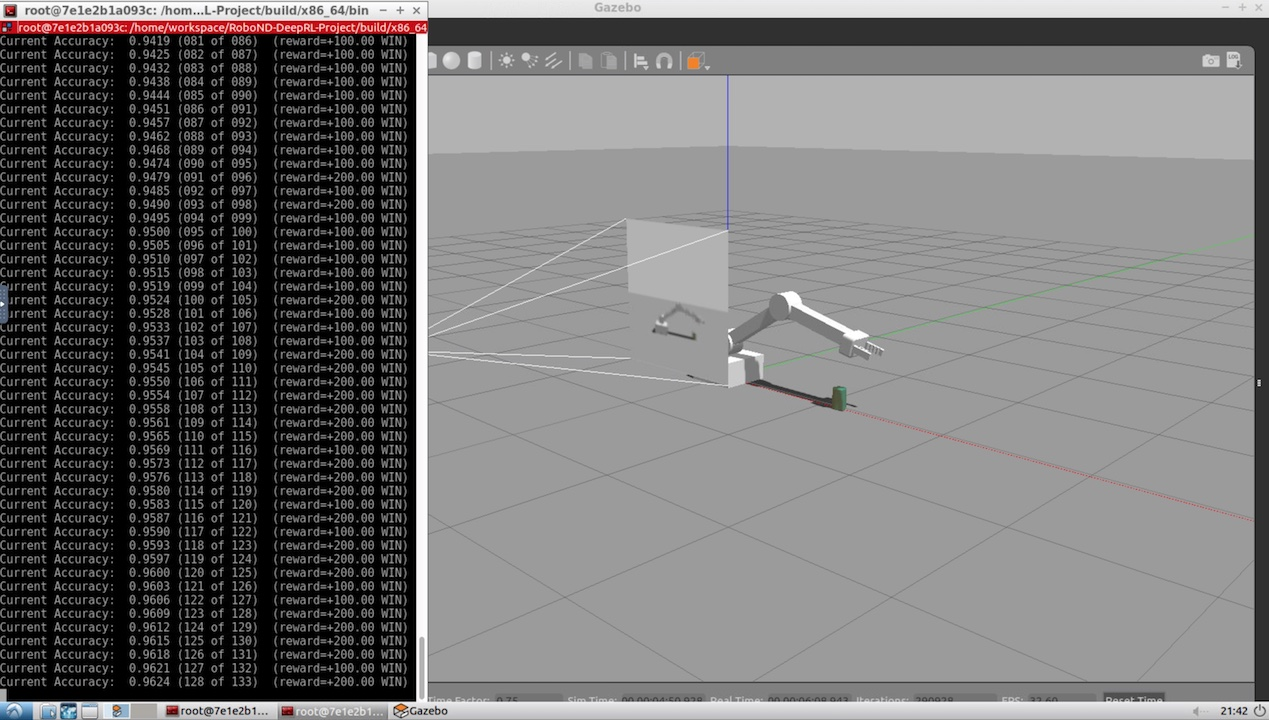
\includegraphics[width=\linewidth]{result-objective1}
    \label{fig:result-objective1}}
  \vfill
  \subfloat[The result for the second objective.]{
  	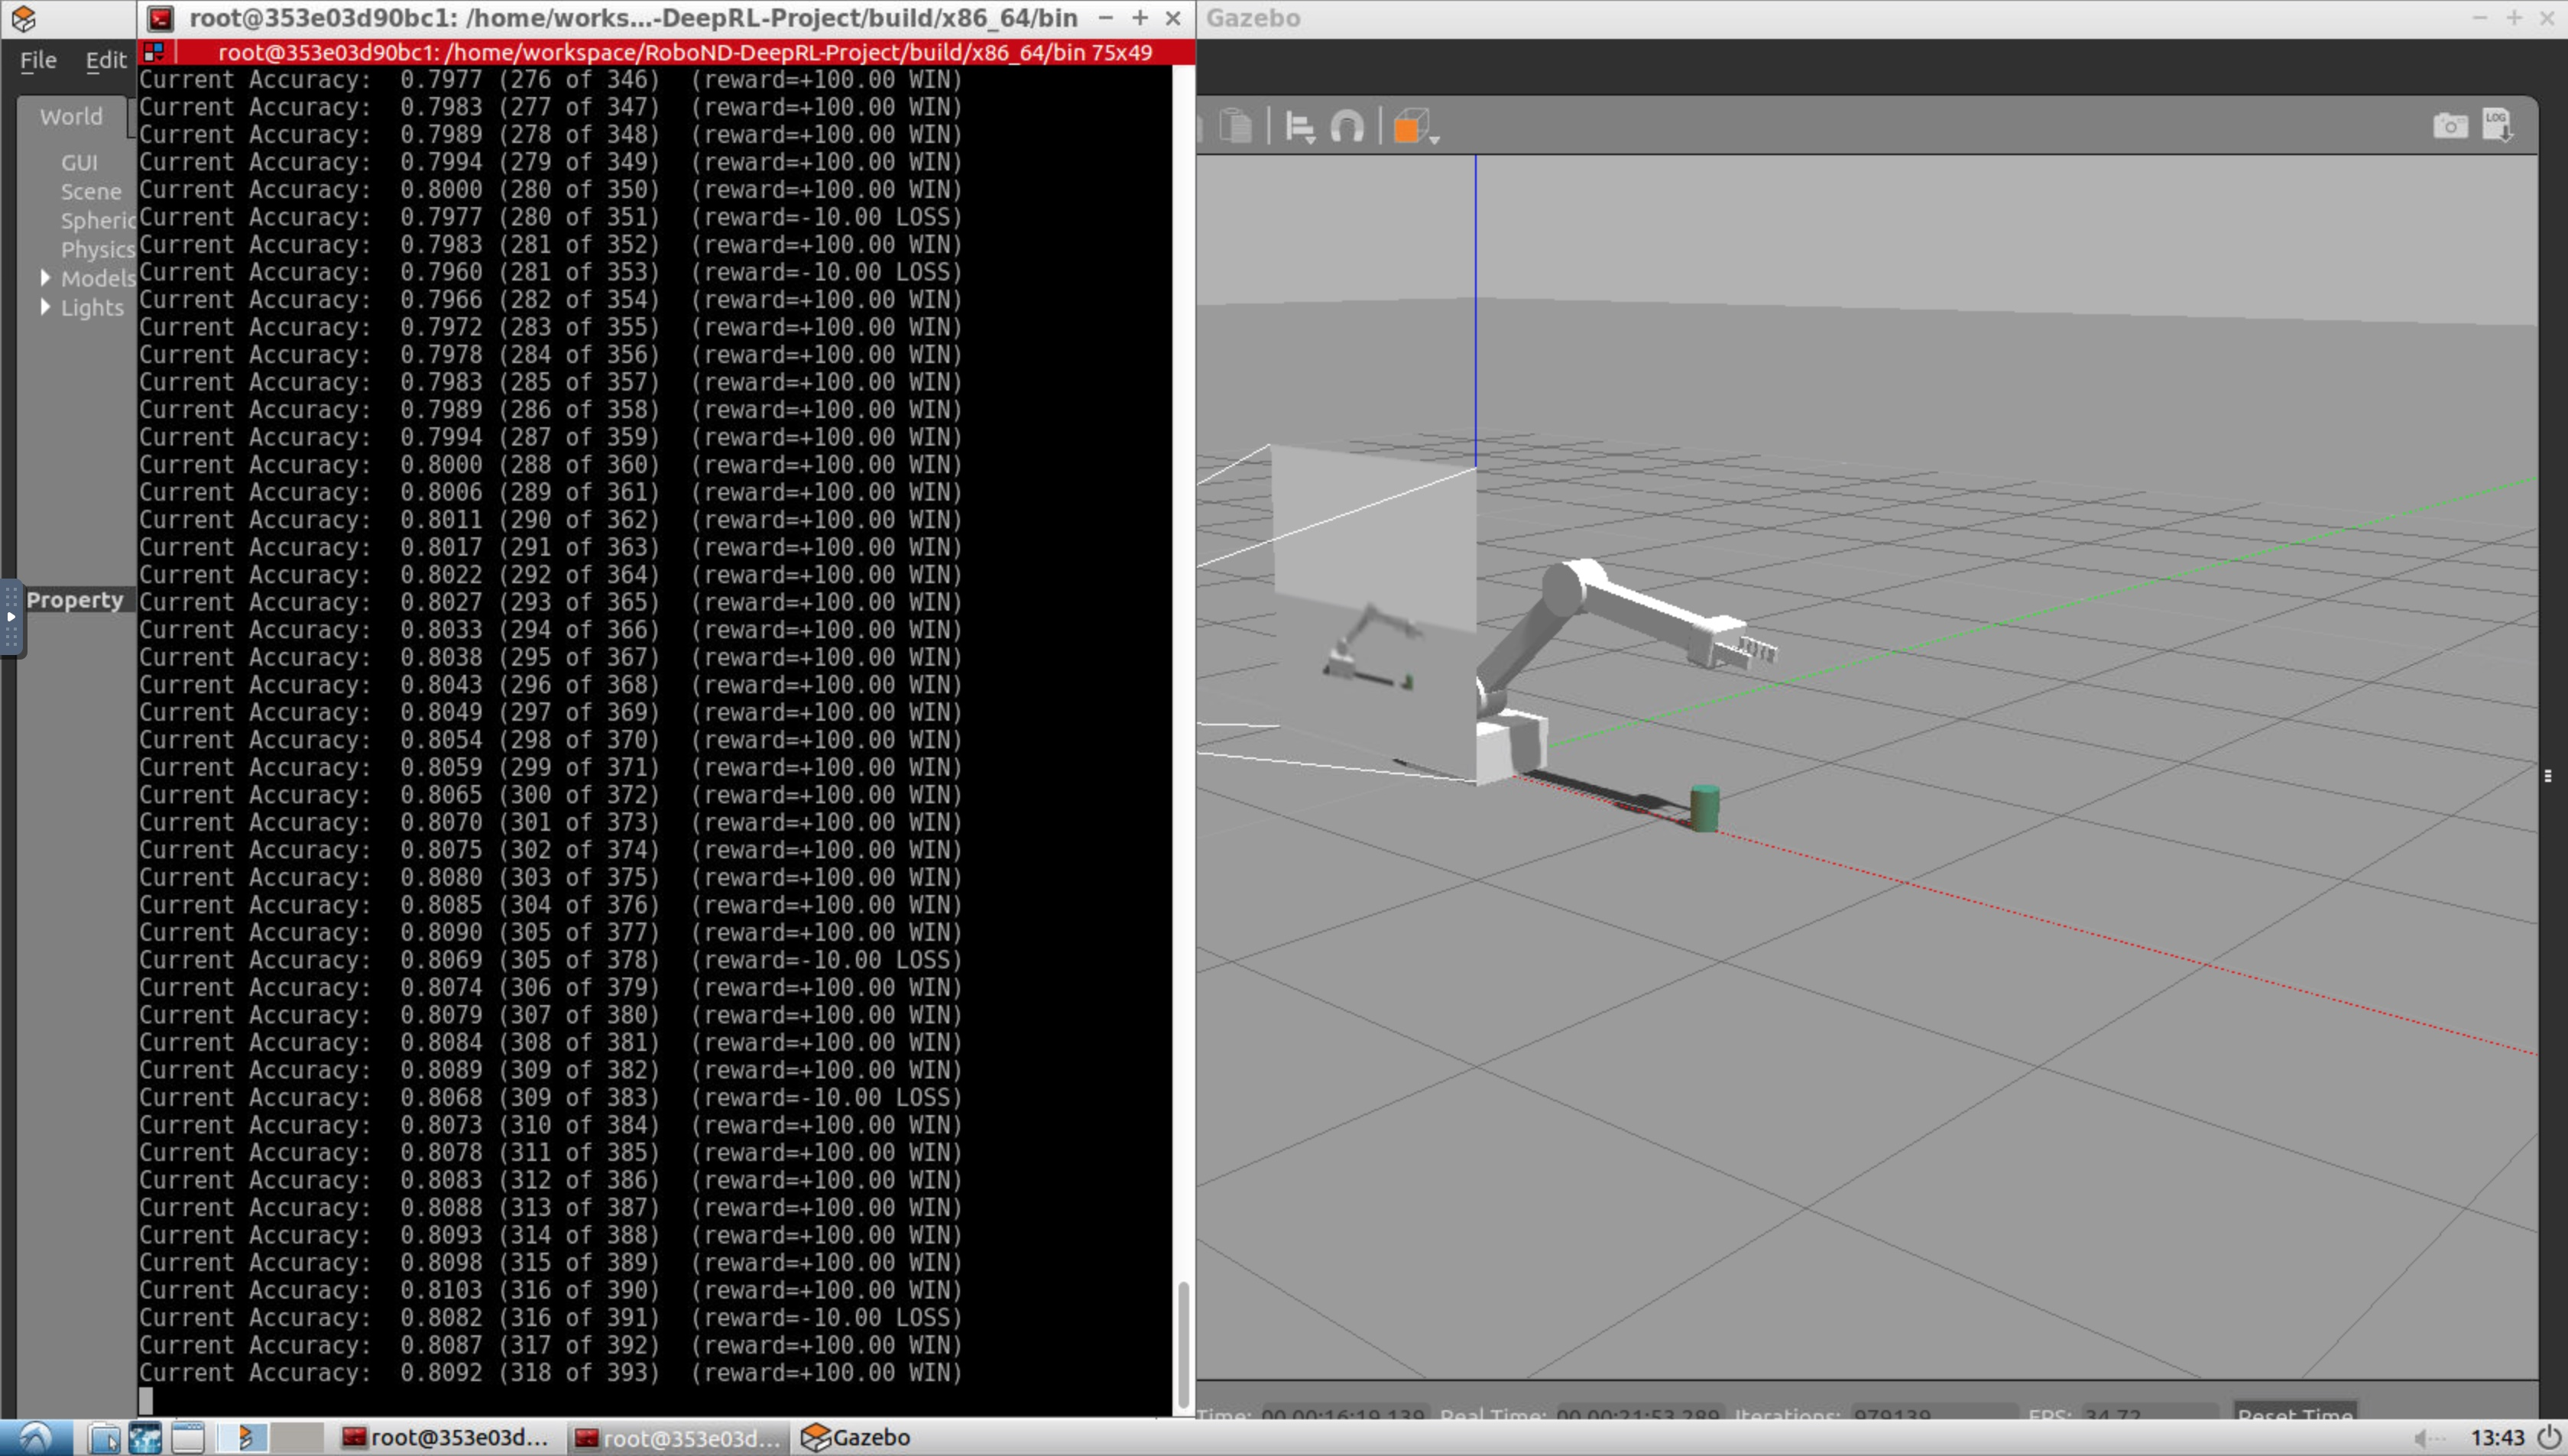
\includegraphics[width=\textwidth]{result-objective2}
    \label{fig:result-objective2}}
  \caption{A screen shot of the result for each objective.}
\end{figure}

\section{Future Work}
Future works include tuning the hyperparameters to address the problem of dependance to the experiences of early episodes, and deal with additional challenges such as randomizing the object position and increasing the arm's degree of freedom.

\bibliographystyle{ieeetr}
\bibliography{bib}

\end{document}